\documentclass[tikz,border=10pt]{standalone}
\usetikzlibrary{intersections, calc}

\begin{document}
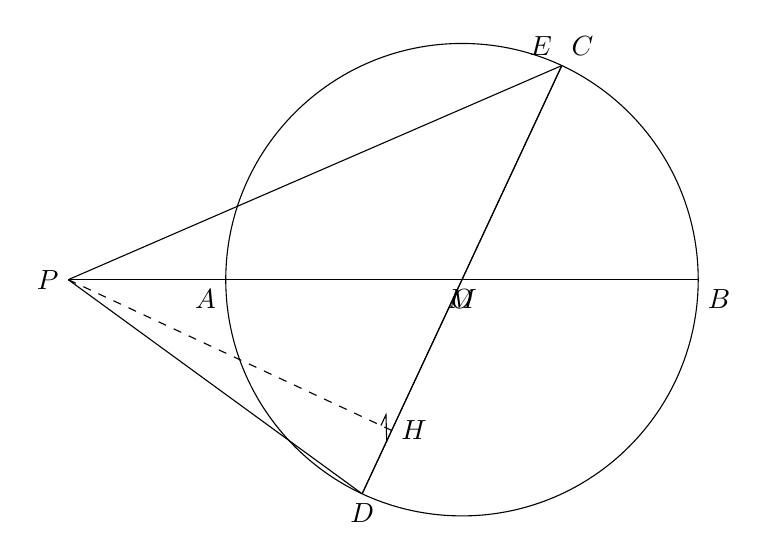
\begin{tikzpicture}
  \def\R{3}
  \coordinate (O) at (0,0);
  \coordinate (P) at (-5,0);
  
  % Circle
  \draw[name path=circle] (O) circle (\R);
  
  % Diameter AB
  \coordinate (A) at (-\R, 0);
  \coordinate (B) at (\R, 0);
  
  % Point C at 65 degrees
  \coordinate (C) at (65:\R);
  
  % Point D opposite to C
  \coordinate (D) at (245:\R);
  
  % Line PC intersects circle at E and C
  \path[name path=PC_line] (P) -- (C);
  \path[name intersections={of=PC_line and circle, by={E, C_dummy}}];
  
  % Line ED intersects AB at M
  \path[name path=ED] (E) -- (D);
  \path[name path=AB_line] (A) -- (B);
  \path[name intersections={of=ED and AB_line, by={M}}];
  
  % Point H: Projection of P on CD
  \coordinate (H) at ($(O)!(P)!(D)$);
  
  % Drawing edges
  \draw (P) -- (B); % P-A-M-O-B
  \draw (P) -- (C); % P-E-C
  \draw (C) -- (D); % C-O-D
  \draw (E) -- (D); % E-M-D
  \draw (P) -- (D); % P-D
  
  % Dashed line PH
  \draw[dashed] (P) -- (H);
  
  % Right angle mark at H
  \draw ($(H)!0.15cm!(P)$) -- ($(H)!0.15cm!(P)!1!90:(H)$) -- ($(H)!0.15cm!(D)$);
  
  % Labels
  \node[left] at (P) {$P$};
  \node[below left] at (A) {$A$};
  \node[below] at (M) {$M$};
  \node[below] at (O) {$O$};
  \node[below right] at (B) {$B$};
  \node[above left] at (E) {$E$};
  \node[above right] at (C) {$C$};
  \node[below] at (D) {$D$};
  \node[right] at (H) {$H$};
  
\end{tikzpicture}
\end{document}
